\documentclass[tikz,border=1.35mm]{standalone}
\usetikzlibrary{arrows.meta}

\definecolor{externalface}{HTML}{8FB9E8}
\definecolor{centroidgreen}{HTML}{0E8814}

% Exploded view of cell-based isotropic refinement for a triangular prism.
% Each original face becomes the base of a pyramid whose apex is a duplicated
% copy of the volume centroid.
\begin{document}
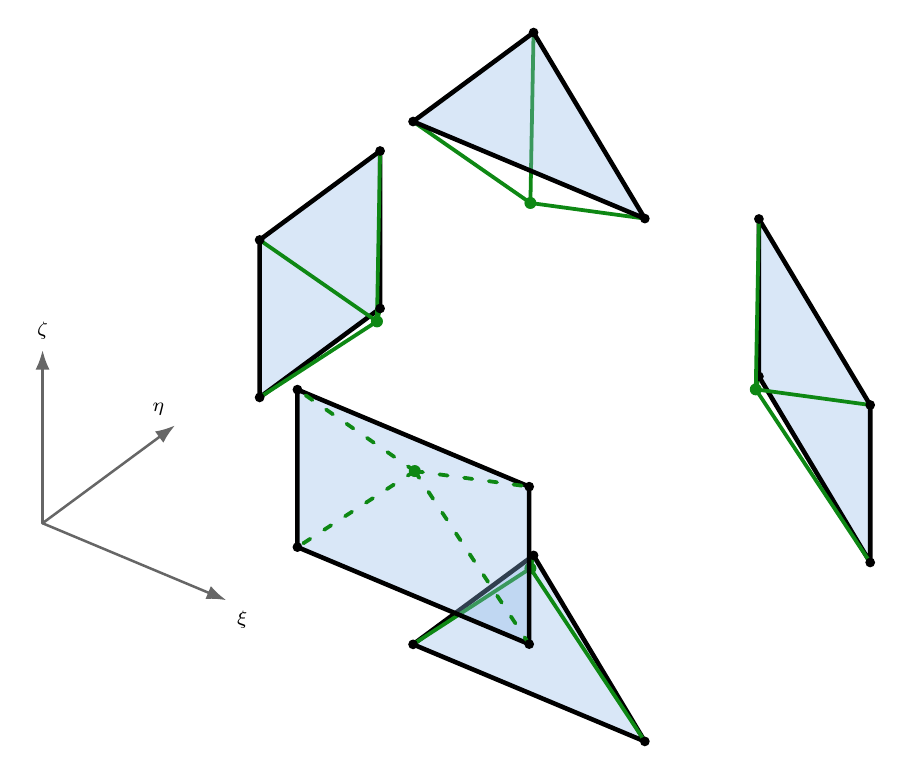
\begin{tikzpicture}[
  x={(20.3mm,-8.5mm)},
  y={(15.3mm,11.3mm)},
  z={(0mm,20mm)},
  line join=round,
  line cap=round,
  outer/.style={draw=black,line width=0.58mm},
  cellface/.style={fill=externalface,fill opacity=0.34,draw=none},
  centroidedge/.style={draw=centroidgreen,line width=0.48mm},
  hiddencentroidedge/.style={draw=centroidgreen,line width=0.48mm,loosely dashed},
  axis/.style={draw=black!60,line width=0.32mm,-{Latex[length=2.5mm,width=1.8mm]}}
]
  \newcommand{\drawtripyramid}[4]{%
    \foreach \p in {#1,#2,#3} {
      \draw[centroidedge] (#4) -- (\p);
    }
    \path[cellface] (#1) -- (#2) -- (#3) -- cycle;
    \draw[outer] (#1) -- (#2) -- (#3) -- cycle;
    \foreach \p in {#1,#2,#3} {
      \fill[black] (\p) circle[radius=0.62mm];
    }
    \fill[centroidgreen] (#4) circle[radius=0.76mm];
  }

  \newcommand{\drawtripyramidgreenfront}[4]{%
    \path[cellface] (#1) -- (#2) -- (#3) -- cycle;
    \draw[outer] (#1) -- (#2) -- (#3) -- cycle;
    \foreach \p in {#1,#2,#3} {
      \draw[centroidedge] (#4) -- (\p);
      \fill[black] (\p) circle[radius=0.62mm];
    }
    \fill[centroidgreen] (#4) circle[radius=0.76mm];
  }

  \newcommand{\drawquadpyramid}[5]{%
    \foreach \p in {#1,#2,#3,#4} {
      \draw[centroidedge] (#5) -- (\p);
    }
    \path[cellface] (#1) -- (#2) -- (#3) -- (#4) -- cycle;
    \draw[outer] (#1) -- (#2) -- (#3) -- (#4) -- cycle;
    \foreach \p in {#1,#2,#3,#4} {
      \fill[black] (\p) circle[radius=0.62mm];
    }
    \fill[centroidgreen] (#5) circle[radius=0.76mm];
  }

  \newcommand{\drawquadpyramidgreenfront}[5]{%
    \path[cellface] (#1) -- (#2) -- (#3) -- (#4) -- cycle;
    \draw[outer] (#1) -- (#2) -- (#3) -- (#4) -- cycle;
    \foreach \p in {#1,#2,#3,#4} {
      \draw[centroidedge] (#5) -- (\p);
      \fill[black] (\p) circle[radius=0.62mm];
    }
    \fill[centroidgreen] (#5) circle[radius=0.76mm];
  }

  \newcommand{\drawquadpyramidhiddengreen}[5]{%
    \path[cellface] (#1) -- (#2) -- (#3) -- (#4) -- cycle;
    \draw[outer] (#1) -- (#2) -- (#3) -- (#4) -- cycle;
    \foreach \p in {#1,#2,#3,#4} {
      \draw[hiddencentroidedge] (#5) -- (\p);
      \fill[black] (\p) circle[radius=0.62mm];
    }
    \fill[centroidgreen] (#5) circle[radius=0.76mm];
  }

  % Compact orientation axes, tucked away from the exploded cells.
  \coordinate (Oaxis) at (-1.70,-0.82,-0.65);
  \draw[axis] (Oaxis) -- (-0.55,-0.82,-0.65) node[below right,font=\scriptsize] {$\xi$};
  \draw[axis] (Oaxis) -- (-1.70,0.28,-0.65) node[above left,font=\scriptsize] {$\eta$};
  \draw[axis] (Oaxis) -- (-1.70,-0.82,0.45) node[above,font=\scriptsize] {$\zeta$};

  % Triangular end-face pyramids.
  \begin{scope}[shift={(0,0,-1.16)}]
    \coordinate (A) at (0,0,0);
    \coordinate (B) at (1.45,0,0);
    \coordinate (C) at (0,1,0);
    \coordinate (O) at (0.483,0.333,0.5);
    \drawtripyramidgreenfront{A}{B}{C}{O}
  \end{scope}

  \begin{scope}[shift={(0,0,1.16)}]
    \coordinate (D) at (0,0,1);
    \coordinate (E) at (1.45,0,1);
    \coordinate (F) at (0,1,1);
    \coordinate (O) at (0.483,0.333,0.5);
    \drawtripyramid{D}{E}{F}{O}
  \end{scope}

  % Side-face pyramids. Each scope moves one original face away from the prism.
  \begin{scope}[shift={(0,-0.96,0)}]
    \coordinate (A) at (0,0,0);
    \coordinate (B) at (1.45,0,0);
    \coordinate (E) at (1.45,0,1);
    \coordinate (D) at (0,0,1);
    \coordinate (O) at (0.483,0.333,0.5);
    \drawquadpyramidhiddengreen{A}{B}{E}{D}{O}
  \end{scope}

  \begin{scope}[shift={(-0.96,0,0)}]
    \coordinate (A) at (0,0,0);
    \coordinate (D) at (0,0,1);
    \coordinate (F) at (0,1,1);
    \coordinate (C) at (0,1,0);
    \coordinate (O) at (0.483,0.333,0.5);
    \drawquadpyramidgreenfront{A}{D}{F}{C}{O}
  \end{scope}

  \begin{scope}[shift={(0.92,0.65,0)}]
    \coordinate (B) at (1.45,0,0);
    \coordinate (C) at (0,1,0);
    \coordinate (F) at (0,1,1);
    \coordinate (E) at (1.45,0,1);
    \coordinate (O) at (0.483,0.333,0.5);
    \drawquadpyramidgreenfront{B}{C}{F}{E}{O}
  \end{scope}
\end{tikzpicture}
\end{document}
